\begin{frame}{Roofnet (Cambridge, MA, 2005)}
{\fontsize{9}{10}\selectfont Bicket, Aguayo, Biswas, Morris, ``Architecture and Evaluation of
an Unplanned 802.11b Mesh Network (MobiCom'05)}
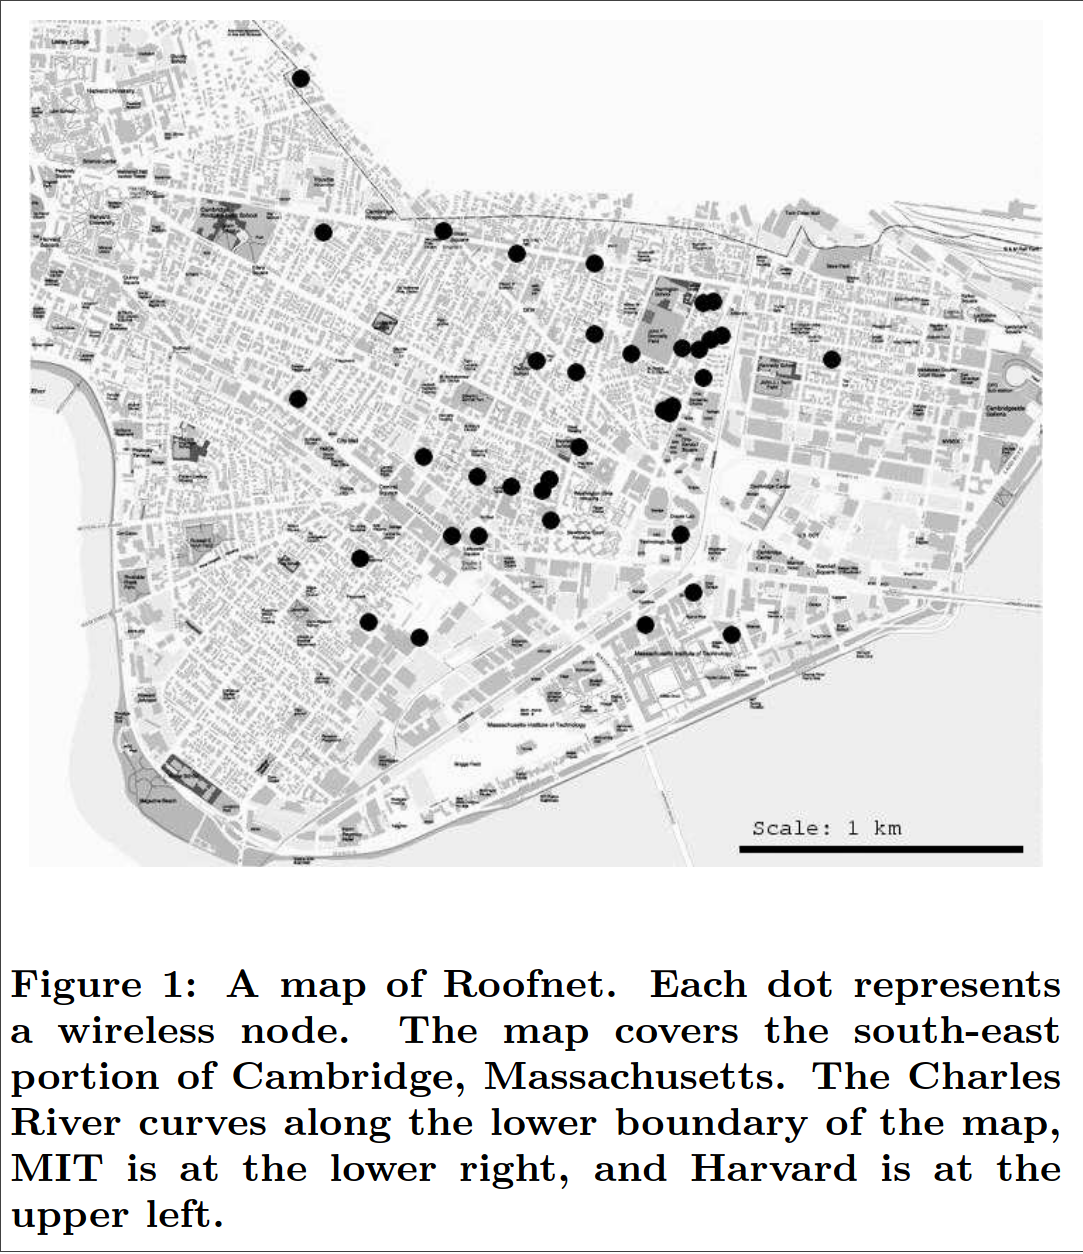
\includegraphics[height=0.8\textheight]{../multiaccess/roofnet-fig1}
\end{frame}

\begin{frame}{roofnet routing}
    \begin{itemize}
    \item up to five hops for packet to get from one node to another
    \item link-state routing protocol between nodes
        \begin{itemize}
        \item no explicit configuration needed
        \end{itemize}
    \item sending nodes computed list of hops + included in packet
        \begin{itemize}
        \item idea called ``source routing''
        \item prevents transient routing loops
        \item important because conditions (e.g. weather) changes connectivity
        \end{itemize}
    \item everyone using same channel!
    \end{itemize}
\end{frame}

\begin{frame}{link-state/distance vector for wireless}
    \begin{itemize}
    \item no explicit list of links/networks
    \item instead: periodically broadcast and see who responds
    \item keep track of signal strength/reliabliy/etc. for routing metrics
    \end{itemize}
\end{frame}

\begin{frame}{modern mesh networks}
    \begin{itemize}
    \item common for distribution network between APs to be (partly) wireless
    \item sysadmin view:
        \begin{itemize}
        \item plug some APs into internet connection
        \item put other APs in appropriate place
        \item APs figure out how to make it work
        \end{itemize}
    \vspace{.5cm}
    \item typically using self-organizing mesh network ideas
        \begin{itemize}
        \item likely similar routing protocols to what we discussed
        \end{itemize}
    \item usually properietary networking protocols
        \begin{itemize}
        \item vendor lock-in problem
        \item (though there is now a recent Wifi standard)
        \end{itemize}
    \end{itemize}
\end{frame}


